\section{Overview}
\label{ch:sieve:sect:overview}

This section presents the two main challenges \tool\ aims
to address and its design rationale and architecture.

\subsection{Design rationale}

As described in Chapter~\ref{chapter:redblue}, adapting applications
to RedBlue consistency requires the programmer to generate
commutative shadow operations and identify which shadow operations can be blue (weakly
consistent) and which must be red (strongly consistent). Thus, to make
this model easy-of-use, the goal of \tool\ is to automate these two tasks, to the extent possible.

With regard to the first task, we leverage the rich commutative replicated data type (CRDT)
literature~\cite{Shapiro2011Conflict,Preguica2009CRDT}, which
defines a list of data types whose operations commute. CRDTs can
be employed to produce commutative shadow operations that converge to identical
final states, independent of the order in which they are applied. 
Shadow operations are thus constructed as a sequence of updates to CRDT data
types that commute by construction.

The challenge in developing shadow operations based on CRDTs is that
the programmer must explicitly transform the applications to replace
all the application state mutations by calls to the
appropriate CRDT object. This involves not only identifying the parts
of the programs that encode these actions, but also understanding the
catalogue of CRDT structures and choosing the appropriate one.  To
minimize this programmer intervention, we 
focus on two-tier architectures that store all of the state that must
persist across operations in a database. This gives us two main
advantages: (1) We can automatically identify the actions that
mutate the state, namely the operations that access the
database. (2) We can reduce the user intervention to small
annotations in the database data organization regarding how to reconcile concurrent updates
to different data items.

The second challenge \tool\ addresses is automatically
labeling commutative shadow operations. To this end, for each shadow operation that is
generated, we only need to decide whether it is invariant safe, according to the
definition in Section~\ref{ch:redblue:sect:shadowops}. (Commutativity does not need
to be checked since the previous step ensures that shadow operations
commute by design.) To automate the classification
process, there are two design alternatives that
represent two ends of a spectrum: (1) a dynamic solution, which determines
at runtime, when the shadow operation is produced, whether that
shadow operation meets the invariant safety property, and (2) a
fully static solution that determines which combinations of initial operation
types, parameters, and initial states they are applied against lead to
generating a shadow operation that is invariant safe.
The problem with the former solution is that it
introduces runtime overheads, and the problem with the latter solution, as
we will detail in Section~\ref{ch:sieve:sec:label}, is
that the static analysis could be expensive and end up conservatively
flagging too many operations as strongly consistent.

To strike a balance between the two approaches, we split the labeling
into a potentially expensive static part and a lightweight dynamic part.
Statically, we generate a set of templates corresponding to different
possible combinations of CRDT operations that comprise shadow operations,
along with weakest preconditions for each template to be invariant
safe. Then, at runtime, we perform a simple dictionary lookup
to determine which
template the shadow operation falls into, so that we can retrieve
the corresponding weakest precondition and determine whether it is met.
%The challenge is how to
%statically analyze the operation code in order to produce this
%dictionary in a way that it: (1) is efficient to look up at runtime,
%(2) has a manageable amount of state, and (3) captures the key
%properties that are required by shadow operations to be
%invariant-preserving, so that it generates no false positives and few
%false negatives in terms of stating that an operation meets this property.

\begin{figure}[t!]
  \centering
  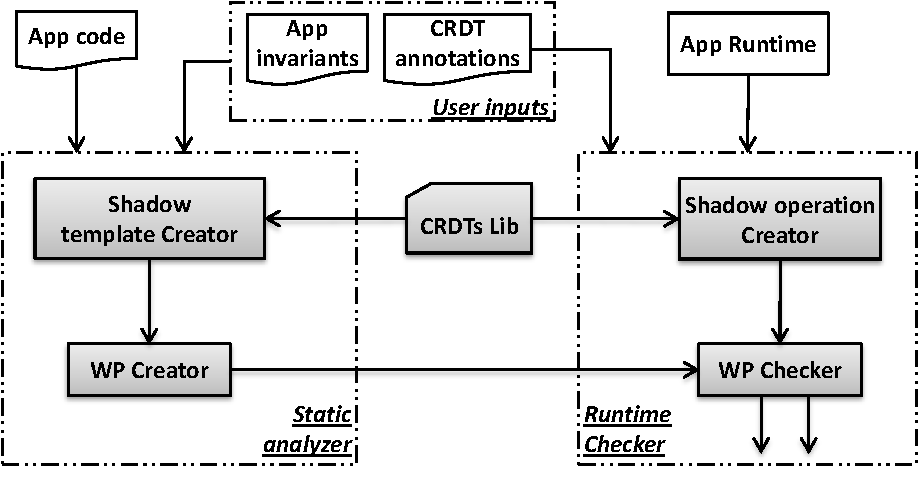
\includegraphics[width=0.85\textwidth]{./figures/sieve/sievearchitecture.pdf}
  \caption{Overview of \tool. Shaded boxes are system components comprising \tool. (WP stands for weakest precondition.)}
  \label{fig:overview}
\end{figure}

\subsection{\tool\ architecture}
These two main solutions above lead to the high level
system architecture depicted in Figure~\ref{fig:overview}. The application
programmer writes the {\em application code} as a series of transactions
written in Java, which access a database
for storing persistent state. Beyond the application code, the only additional
inputs that the programmer needs to provide are {\em CRDT annotations}
specifying the semantics for merging concurrent updates and 
a set of application-specific invariants.
The static analyzer then 
creates {\em shadow operation templates} from the code of each transaction,
where these templates represent different sequences of invocations of
functions in a {\em CRDT library}. The analyzer also
computes the  {\em weakest preconditions} required for each template
to be invariant safe. 

At runtime, application servers run both the Java logic and 
the {\em runtime checker}, and interact with a database server (not shown in the figure)
and the replication tier (not shown in the figure).
%are deployed at each site or each replica within a single site. 
While executing a transaction, the application server runs the
generator operation \changebars{and accumulates side effects in a {\em shadow operation creator}.
Upon commit called by the generator, }{inside a {\em shadow operation creator}, which,} instead of
directly committing side effects to the database, \changebars{the {\em creator}}{} 
generates a shadow operation consisting of a sequence of 
invocations from the CRDT library.
This shadow operation is then fed to the {\em weakest
precondition checker} to decide which static template it falls into, 
and what is the precondition required for
the operation to be invariant safe, which allows the runtime to
determine how to label the operation. The labeled shadow operation is then fed to
the replication system implementing multi-level consistency.
In the following sections we further detail the design and implementation
of the main components of this architecture.
%The overall architecture of
%the tool we built is shown in Figure~\ref{fig:overview}. It is
%comprised of two major components: namely (a) static analysis and (b)
%runtime logic.

%% %\paragraph{Workflow:}
%% %{\em RR: This paragraph is going into too much detail and introducing
%% %terminology that wasn't used before. Needs to be written at a higher level.}
%% Taking the source code of applications as input,
%% together with the invariants that need to be preserved and
%% the schema annotations regarding the conflict resolution semantics,
%% the static analyzer generates a series of templates describing
%% the shadow operations that may be produced at runtime, and produces
%% a dictionary that can be looked up at runtime to efficiently
%% determine which template each generated shadow operation corresponds
%% to. Furthermore, the static analysis produces a series
%% of weakest preconditions required for
%% an instantiation of each of these templates to meet the invariant
%% preservation property.
%% % the path extractor
%% %generates a path abstraction (regular expression) for each
%% %transaction. The path analyzer reduces each path abstraction into a
%% %set of reduced path abstractions (regular expression without $*$ and
%% %$|$ operators). Next, the template creator generates a shadow
%% %operation template for each control flow represented by a reduced path
%% %abstraction. The last step of the static analysis is to ask Jahob to
%% %compute the weakest precondition for each shadow operation template.
%% The output by this static analysis is then used by the runtime
%% logic as follows. Upon the arrival of a user request, the initial
%% operation is invoked by the shadow operation creator, which also
%% looks up the dictionary to determine which template the generated
%% shadow operation falls into. 
%% Once the shadow operation is produced and the dictionary lookup
%% determines the corresponding template, the creator will look up
%% the weakest precondition corresponding to that template
%% and determine if the operation parameters meet this weakest precondition
%% in order to determine the correct color.


\if 0
%% In order to achieve the vision outlined above, there are specific
%% difficulties that must be overcome. \rodrigo{The first three are
%% interconnected, the differences might be too subtle to be made
%% so explicitly at this point. The last one is specific to an
%% aspect of the solution, which is that we are using path info to
%% look up the dictionary.}
%% \begin{enumerate}
%% \item The dictionary must be efficient to look up and any
%%   post-processing after the lookup must be efficient to perform
%% \item The dictionary must be a mangeable size to not bloat the
%%   run-time overheads of the system
%% \item A sensible look-up key must be identified at runtime and used to seed the dcitionary
%% \item The potentially infinite series of executions correspnoding to
%%   loops must be addressed without enumerating all possible loops (and
%%   exploding teh dictionary).
%% \end{enumerate}

%% \allen{figure missing to demonstrate the architecture}

%% \rodrigo{Need to give overview of how system works: dictionary is
%% produced offline, at runtime operation is invoked at a site, generates
%% shadow in parallel with dictionary lookup, this leads to coloring
%% shadow, which is conveyed to the RedBlue platform for the appropriate
%% replication to take place.}

%% The subsequent sections are devoted to describing the design and
%% implementation of the run-time system for generating shadow operations
%% and the static analysis used to build the red-blue dictionary.
\fi
